\chapter{Core Concepts}
The HTTP Header fields mainly used to carry out desynchronization attacks are \textsc{Content-Length} and \textsc{Transfer-Encoding: chunked}. There are two combinations possible : 
\section{Using two Content-Length header fields:}
	This technique is very simple but is rarely effective as most of the modern systems are designed to selectively reject any requests with multiple \textsc{Content-Length} headers.\\
	Below is an example HTTP request, referenced from \cite{b6}:
	\begin{verbatim}
	POST / HTTP/1.1
	Host: example.com
	Content-Length: 6
	Content-Length: 5
	\end{verbatim}
\section{Using combination of Content-Length and Transfer-Encoding: chunked header fields:}This technique can be used to realize practical attacks in real environments. 
	Below is an example request, referenced from \cite{b6}:
	\begin{verbatim}
	POST / HTTP/1.1
	Host: example.com
	Content-Length: 3
	Transfer-Encoding: chunked
	\end{verbatim}
	This technique is valid as per the specifications in RFC 2616\cite{b10} which states : \\
	\textit{"If a message is received with both a Transfer-Encoding header field and a Content-Length header field, the latter MUST be ignored".}\\
	The core idea here is to hide the \textsc{Transfer-Encoding:chunked} header field from atleast one system in a chain of systems. It will make sure that the \textsc{Content-Length} header is used as a fallback and this will allow us to desynchronize the whole system.

We can explain this technique using two simple examples : 
\begin{itemize}
	\item Take a look at the example in figure \ref{fig:Frontend} which is referenced from \cite{b6}:
	If the frontend doesn't support chunked encoding, this kind of a request can be sent. Every chunk is constituted by a chunk size, followed by a new line character and then the actual contents of the chunk. As frontend ignores chunked encoding, the backend considers the \textsc{Content-Length} header, appending the malicious message to the next request and thus desynchronizing the system.
\end{itemize}

\begin{figure}
	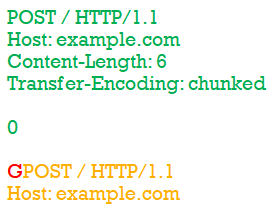
\includegraphics{images/Frontend}
	\caption{Frontend}
	\label{fig:Frontend}
\end{figure} 

\begin{itemize}
	\item Take a look at the example in figure \ref{fig:Backend} which is referenced from \cite{b6}: This kind of request is helpful when the backend ignores chunked encoding. The logic works same as described for frontend.
\end{itemize}
\begin{figure}
	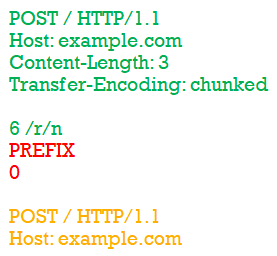
\includegraphics{images/Backend}
	\caption{Backend}
	\label{fig:Backend}
\end{figure}

Further complex desynchronizations can be achieved by carefully hiding the \textsc{Transfer-Encoding} header field or making it harder to detect. 